%% Creator: Inkscape inkscape 0.48.0, www.inkscape.org
%% PDF/EPS/PS + LaTeX output extension by Johan Engelen, 2010
%% Accompanies image file 'pulse_demo.ps' (pdf, eps, ps)
%%
%% To include the image in your LaTeX document, write
%%   \input{<filename>.pdf_tex}
%%  instead of
%%   \includegraphics{<filename>.pdf}
%% To scale the image, write
%%   \def\svgwidth{<desired width>}
%%   \input{<filename>.pdf_tex}
%%  instead of
%%   \includegraphics[width=<desired width>]{<filename>.pdf}
%%
%% Images with a different path to the parent latex file can
%% be accessed with the `import' package (which may need to be
%% installed) using
%%   \usepackage{import}
%% in the preamble, and then including the image with
%%   \import{<path to file>}{<filename>.pdf_tex}
%% Alternatively, one can specify
%%   \graphicspath{{<path to file>/}}
%% 
%% For more information, please see info/svg-inkscape on CTAN:
%%   http://tug.ctan.org/tex-archive/info/svg-inkscape

\begingroup
  \makeatletter
  \providecommand\color[2][]{%
    \errmessage{(Inkscape) Color is used for the text in Inkscape, but the package 'color.sty' is not loaded}
    \renewcommand\color[2][]{}%
  }
  \providecommand\transparent[1]{%
    \errmessage{(Inkscape) Transparency is used (non-zero) for the text in Inkscape, but the package 'transparent.sty' is not loaded}
    \renewcommand\transparent[1]{}%
  }
  \providecommand\rotatebox[2]{#2}
  \ifx\svgwidth\undefined
    \setlength{\unitlength}{240.26850586pt}
  \else
    \setlength{\unitlength}{\svgwidth}
  \fi
  \global\let\svgwidth\undefined
  \makeatother
  \begin{picture}(1,1.26250966)%
    \put(0,0){\includegraphics[width=\unitlength]{pics/pulse_demo.ps}}%
    \put(0.12536247,0.0993745){\color[rgb]{0,0,0}\makebox(0,0)[lb]{\smash{$0$}}}%
    \put(0.26870684,0.0993745){\color[rgb]{0,0,0}\makebox(0,0)[lb]{\smash{$0.5$}}}%
    \put(0.45547157,0.09871443){\color[rgb]{0,0,0}\makebox(0,0)[lb]{\smash{$1$}}}%
    \put(0.59821277,0.0993745){\color[rgb]{0,0,0}\makebox(0,0)[lb]{\smash{$1.5$}}}%
    \put(0.78703737,0.09871443){\color[rgb]{0,0,0}\makebox(0,0)[lb]{\smash{$2$}}}%
    \put(0.92989614,0.0993745){\color[rgb]{0,0,0}\makebox(0,0)[lb]{\smash{$2.5$}}}%
    \put(0.47905735,0.00614547){\color[rgb]{0,0,0}\makebox(0,0)[lb]{\smash{$t$\,(мкс)}}}%
    \put(0.8811366,1.20290176){\color[rgb]{0,0,0}\makebox(0,0)[lb]{\smash{$(а)$}}}%
    \put(0.8811366,0.8252291){\color[rgb]{0,0,0}\makebox(0,0)[lb]{\smash{$(б)$}}}%
    \put(0.8811366,0.43899454){\color[rgb]{0,0,0}\makebox(0,0)[lb]{\smash{$(в)$}}}%
    \put(0.024,0.23179613){\color[rgb]{0,0,0}\rotatebox{90}{\makebox(0,0)[lb]{\smash{$\Delta{}B$\,(мГс)}}}}%
    \put(0.04,0.15673342){\color[rgb]{0,0,0}\makebox(0,0)[lb]{\smash{$-10$}}}%
    \put(0.06,0.30447575){\color[rgb]{0,0,0}\makebox(0,0)[lb]{\smash{$-5$}}}%
    \put(0.09990613,0.48097069){\color[rgb]{0,0,0}\makebox(0,0)[lb]{\smash{$0$}}}%
    \put(0.024,0.58158963){\color[rgb]{0,0,0}\rotatebox{90}{\makebox(0,0)[lb]{\smash{$dB/dt$\,(у.е.)}}}}%
    \put(0.06,0.55166116){\color[rgb]{0,0,0}\makebox(0,0)[lb]{\smash{$-2$}}}%
    \put(0.09990613,0.65597489){\color[rgb]{0,0,0}\makebox(0,0)[lb]{\smash{$0$}}}%
    \put(0.10147664,0.76022787){\color[rgb]{0,0,0}\makebox(0,0)[lb]{\smash{$2$}}}%
    \put(0.09942815,0.86481839){\color[rgb]{0,0,0}\makebox(0,0)[lb]{\smash{$4$}}}%
    \put(0.024,1.00531307){\color[rgb]{0,0,0}\rotatebox{90}{\makebox(0,0)[lb]{\smash{$U$\,(у.е.)}}}}%
    \put(0.06,0.94062602){\color[rgb]{0,0,0}\makebox(0,0)[lb]{\smash{$-2$}}}%
    \put(0.06,1.00446217){\color[rgb]{0,0,0}\makebox(0,0)[lb]{\smash{$-1$}}}%
    \put(0.09990613,1.06771421){\color[rgb]{0,0,0}\makebox(0,0)[lb]{\smash{$0$}}}%
    \put(0.10111246,1.13092073){\color[rgb]{0,0,0}\makebox(0,0)[lb]{\smash{$1$}}}%
    \put(0.10147664,1.19384268){\color[rgb]{0,0,0}\makebox(0,0)[lb]{\smash{$2$}}}%
  \end{picture}%
\endgroup
